\chapter{Transient Absorption in Condensed Matter Samples}

\section{Statement of Contribution}
This experiment uses home-made equipment consisting of a XUV-IR Mach-Zhender interferometer, a bright XUV light source, a target chamber and an XUV photon spectrometer. The entire apparatus is held under vacuum ($10^{-3} - 10^{-9}$ Torr) and was designed, built and tested by Gregory Smith and Stephen Hageman. The LabView software controlling the spectrometer's detector was programmed by Kent Talbert. The vacuum system's safety system was designed and programmed by Andrew Piper. The germanium samples were grown by Dr. Yaguo Tang. Transient absorption experiments were done by Gregory Smith and Stephen Hageman; analysis was done by Gregory Smith. Further details on the apparatus and the relevant physics will be discussed in the main dissertation.

\section{Introduction}

\begin{figure}
	\centering
	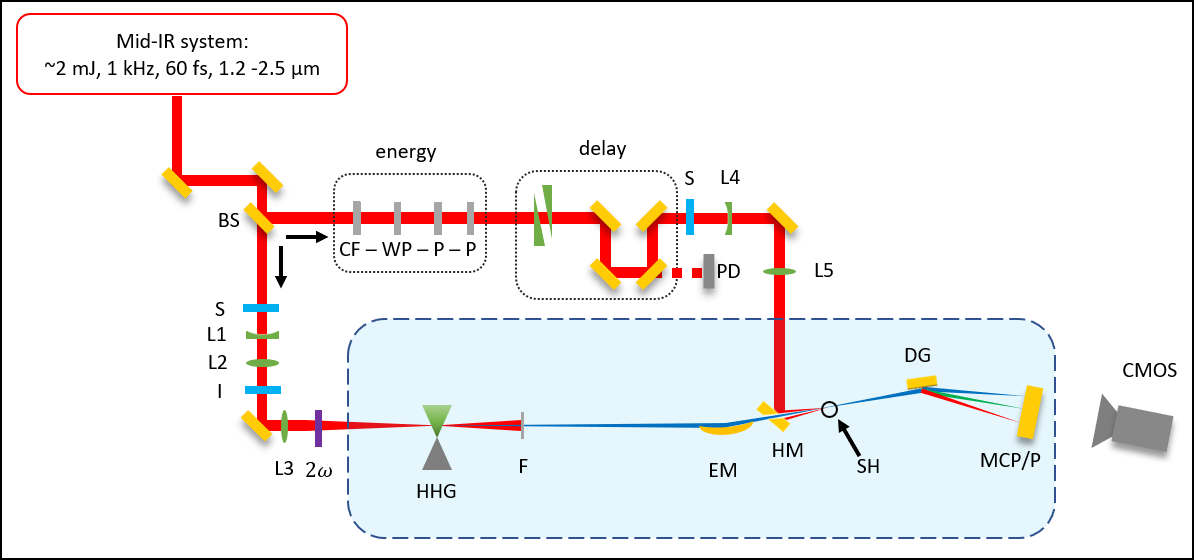
\includegraphics[width=0.95\textwidth]{figures/chap3/beamline_schematic.png}
	\caption{Schematic of the Transient Absorption BeamLine (TABLe). Blue shaded region is under vacuum. BS: beam splitter, L: lens, HHG: high harmonic generation, F: metallic filter, EM: ellipsoidal mirror, HM: hole mirror, PD: photodiode, DG: dispersive grating, MCP/P: micro-channel plate and phosphor.}
	\label{fig:beamline_schematic}
\end{figure}

\begin{figure}
	\centering
	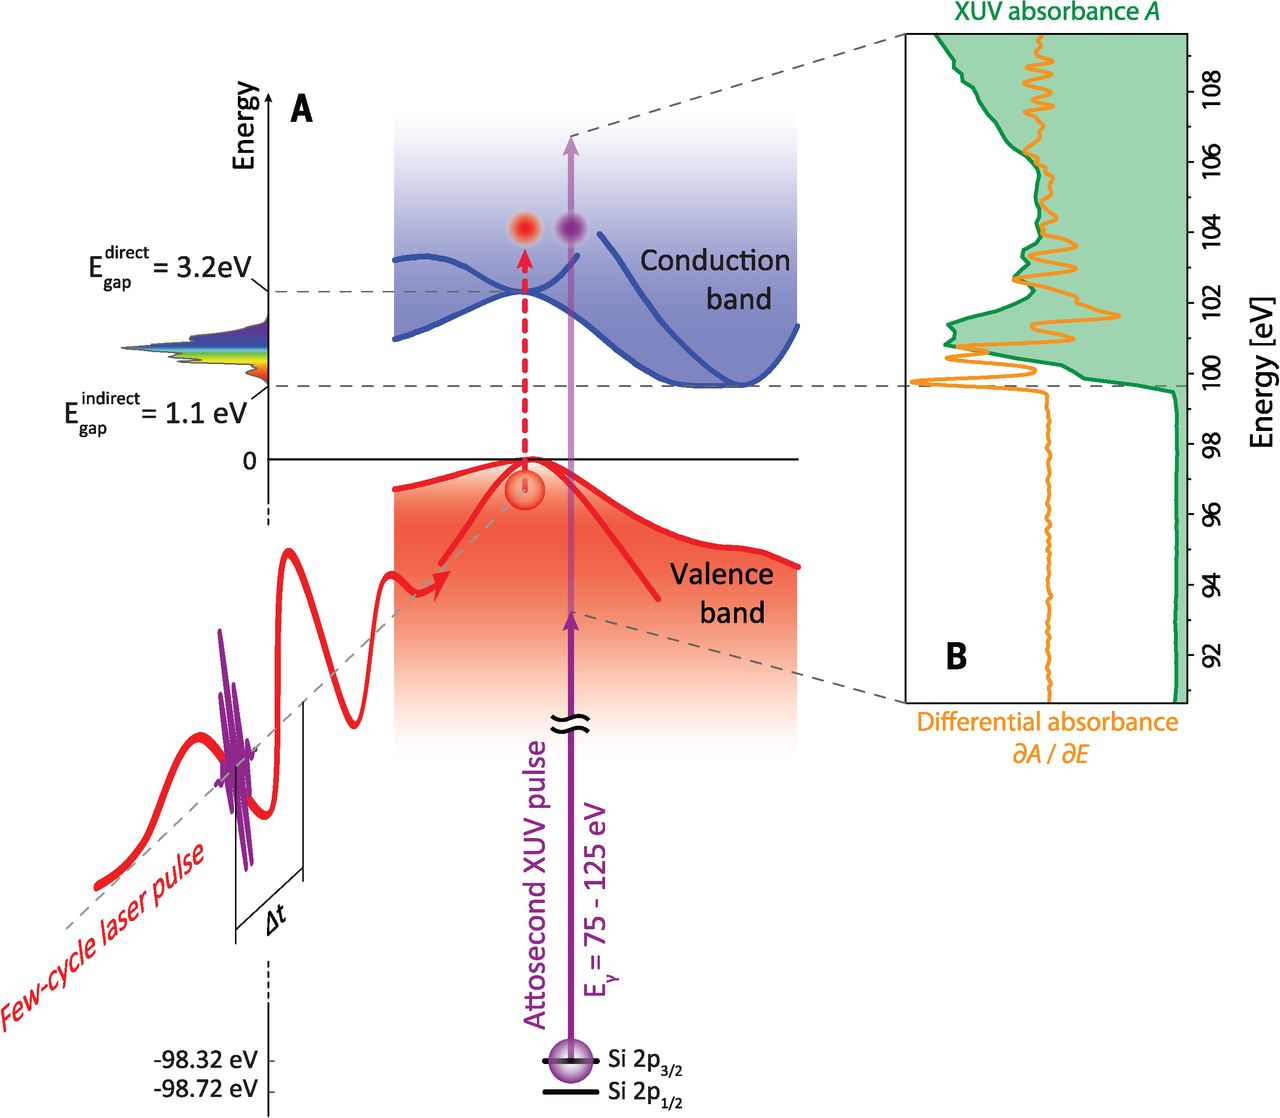
\includegraphics[width=0.75\textwidth]{figures/chap3/ATAS_Cartoon_Si_Leone.jpg}
	\caption{Schematic of an attosecond transient absorption spectroscopy (ATAS) experiment. An IR laser pulse excites electrons in the material, driving them across the band-gap. An XUV pulse passes through the sample after a delay $\Delta t$. The measured XUV absorbance is sensitive to electronic populations and states. Figure taken from \cite{schultzeAttosecondBandgapDynamics2014}.}
	\label{fig:ATAS_Cartoon_Si_Leone}
\end{figure}

We generate extreme ultraviolet (XUV) light using an extremely non-linear process called \textit{high harmonic generation} (HHG). Briefly, the XUV light source can be thought of as a frequency comb spanning from $\sim20$ eV to $\sim50$ eV. The separation between the teeth of the frequency comb is $\omega$, the frequency of our laser light. In the time domain, the XUV is a train of attosecond bursts of broadband light with an envelope of $\sim50$ fs. Due to the ionizing nature of XUV light, the entire experiment must be performed under vacuum.

The experiment is powered by a commercial mid-IR laser system (Spectra Physics Spitfire ACE, Light Conversion HE TOPAS Prime), which delivers $\sim2$ mJ at $100 - 1,000$ Hz repetition rate, $\sim65$ fs duration, $1.2 - 2.5$ $\mu$m wavelength. The output of the TOPAS is routed into a Mach-Zhender interferometer, shown in \cref{fig:beamline_schematic}. A beam splitter (BS) delivers the bulk of the pulse energy ($96\%$) to the generation arm of the interferometer, which contains the HHG source and specialized XUV focusing optics. A small percentage of TOPAS's pulse energy goes to the pump arm, which contains optics to control the pulse energy and relative delay between the two arms. The pump arm also contains a series of lenses that focus the light into the vacuum system. A silvered hole mirror (HM) combines the two arms of the interferometer collinearly. This optic is designed to allow the XUV light to pass through a clear aperture on the backside of the HM while the pump arm's IR light reflects off the front face. The interferometer is aligned so that both arms have a common focus in the target chamber.

The basic concept of an attosecond transient absorption spectroscopy (ATAS) experiment is shown in \cref{fig:ATAS_Cartoon_Si_Leone}. In such an experiment, a sample is placed at the combined XUV/IR focus in a transmission geometry. An XUV photon spectrometer is placed behind the sample and the transmitted XUV spectrum $S$ is measured as a function of IR-XUV delay. The IR light is not measured by the spectrometer.

Absorption features in the spectrum correspond to photoabsorption, which drive electronic transitions. At XUV photon energies, these transitions are from a core-level state to a state near the Fermi level. Since the HHG process produces a near-continuum, the XUV light will drive nearly all allowed transitions within its bandwidth. One of the core assumptions of an ATAS experiment is that the initial core state is shielded from the IR pulse by the valence electrons. However, the valence states are influenced by the external IR field, which causes both a change in electron population among these states, as well as a change in the states themselves. By measuring the XUV spectrum as a function of XUV-IR delay, we can track these electronic transitions - and thus the sample's electron dynamics - in response to an ultrafast optical excitation.

something, something physical motivation. maybe talk about what other measurements have done.

IR=pump, XUV=probe is not strictly true ... but it is a good approximation in solids.

need citations for this discussion.

\section{Sample Requirements and Geometry}

There are several sample requirements for a successful condensed matter transient absorption experiment. First and foremost, the sample needs to have an absorption edge within the bandwidth of the XUV source. Second, the material must be thin enough to transmit XUV at and near the absorption edge, yet thick enough to see small changes in the absorption. Typically, this means the sample will be a free-standing membrane on the order of 10 - 200 nm thick, depending on the material and XUV source brightness. Next, the sample needs to be excitable using laser sources present in our lab (i.e., ultrafast pulses with wavelengths between 800 nm and a couple of microns). To avoid slow build up of heat (on the order of seconds) and laser-induced damage, the sample needs to be rastered through the laser focus as the experiment is performed. This rastering method necessitates both a large clear aperture ($\sim$ 1 mm$^2$ - 1 cm$^2$) and good sample uniformity. Samples that meet the above thickness and clear aperture requirements are extremely delicate, with thicknesses between 5,000 and 100,000 times smaller than their lateral dimensions. As such, one should expect most samples to break before, during and after measurements, and a successful experiment will have a material pipeline that is capable of producing multiple, consistent samples in a short time frame.

\begin{figure}
	\centering
	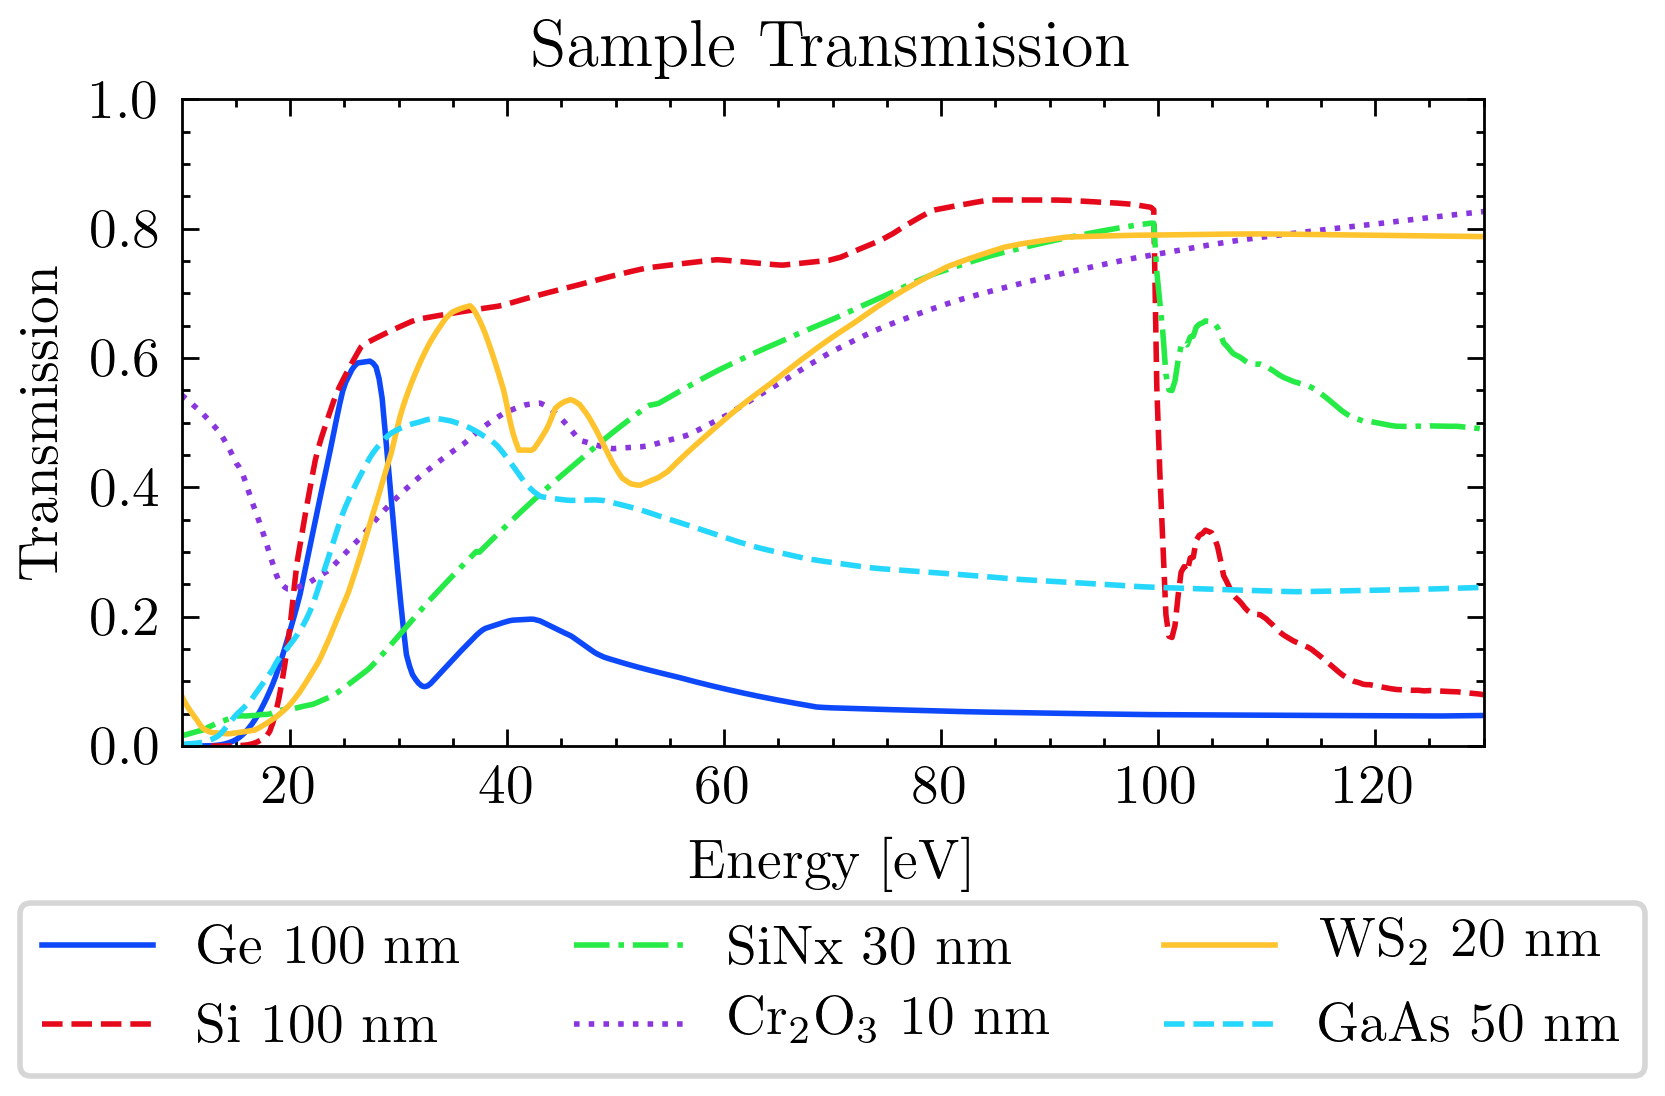
\includegraphics[width=0.5\textwidth]{figures/chap3/Sample_trans_CXRO.png}
	\caption{Expected XUV transmission of various samples. Data calculated from \cite{gulliksonCXROXRayInteractions}.}
	\label{fig:Sample_trans_CXRO}
\end{figure}

\begin{figure}
	\centering
	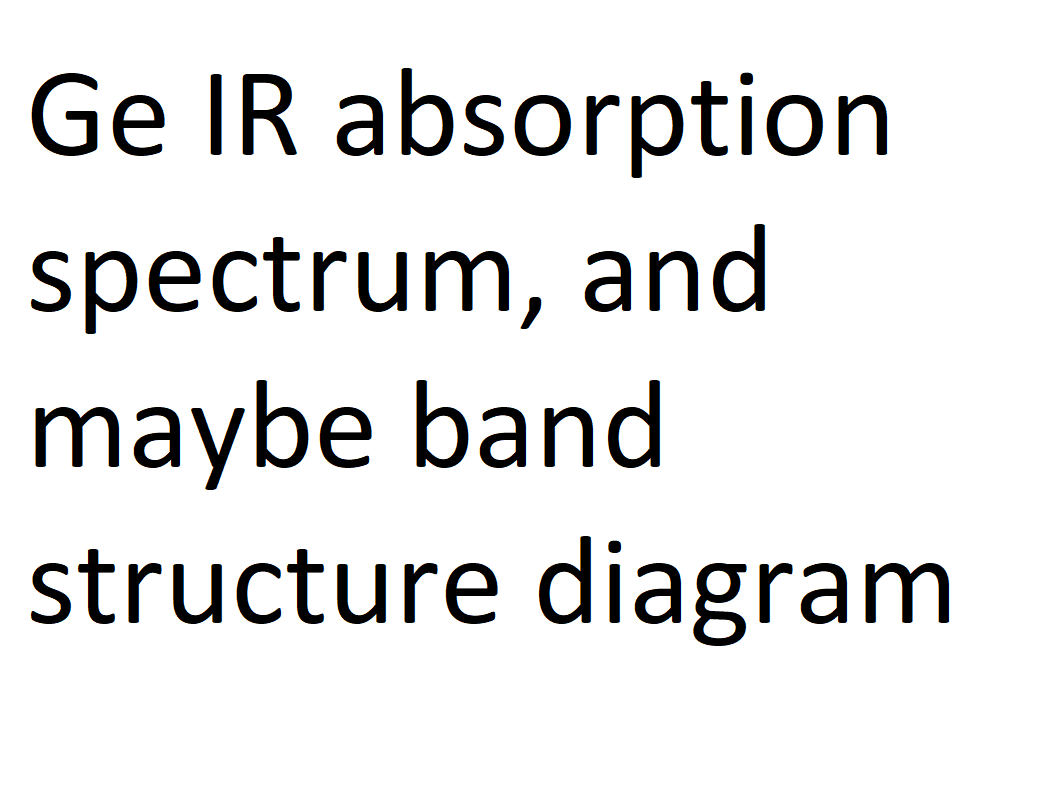
\includegraphics[width=0.5\textwidth]{figures/chap3/Ge_IR_absorption.png}
	\caption{this figure shows the IR absorption of germanium and the band structure, from the literature. (citation)}
	\label{fig:Ge_IR_absorption}
\end{figure}


\section{Data Collection}

\begin{figure}
	\centering
	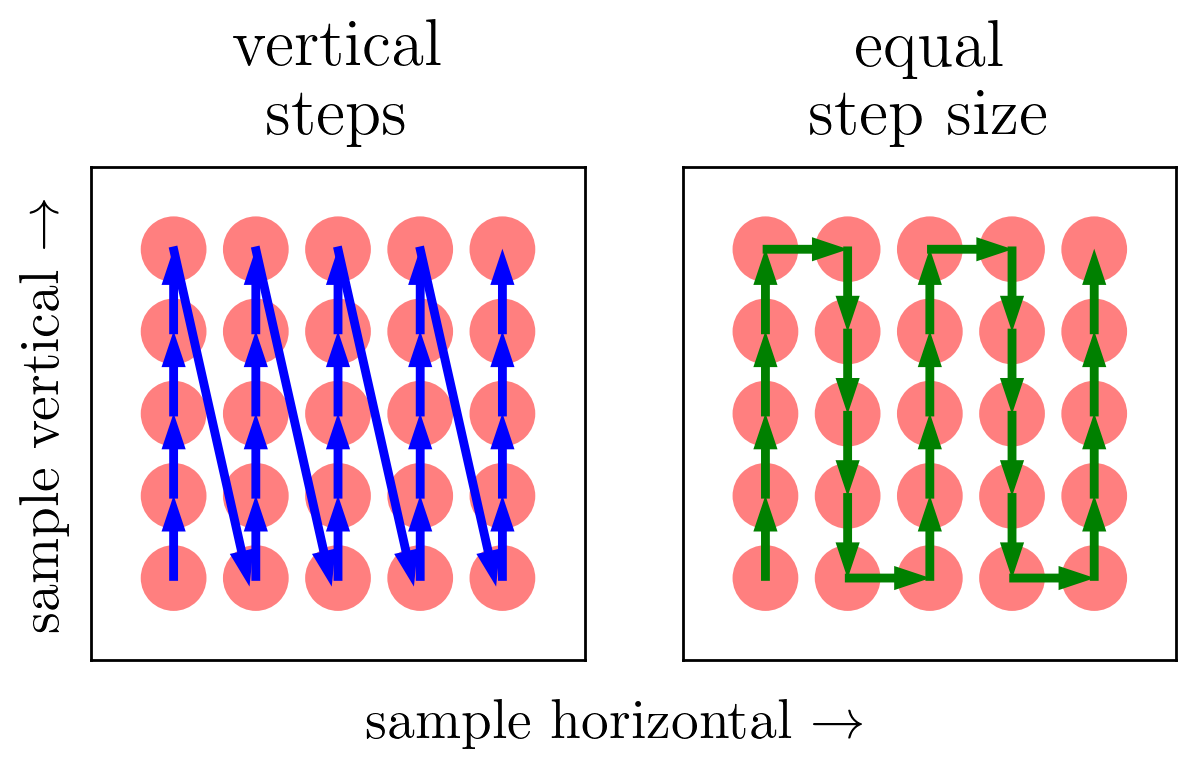
\includegraphics[width=0.75\textwidth]{figures/chap3/Rastering_Methods.png}
	\caption{Schematic showing competing raster methods. The clear aperture of the sample is represented by the border of the black square. The laser focal spots are shown as red circles, and the movement of the sample holder relative to the laser focus is indicated by arrows. The method in the left panel yields more repeatable positioning, but has a bimodal distribution of motor transit times. The method shown in the right panel has equal step size for all movements, resulting in a tighter distribution of transit times.}
	\label{fig:Rastering_Methods}
\end{figure}

\begin{figure}
	\centering
	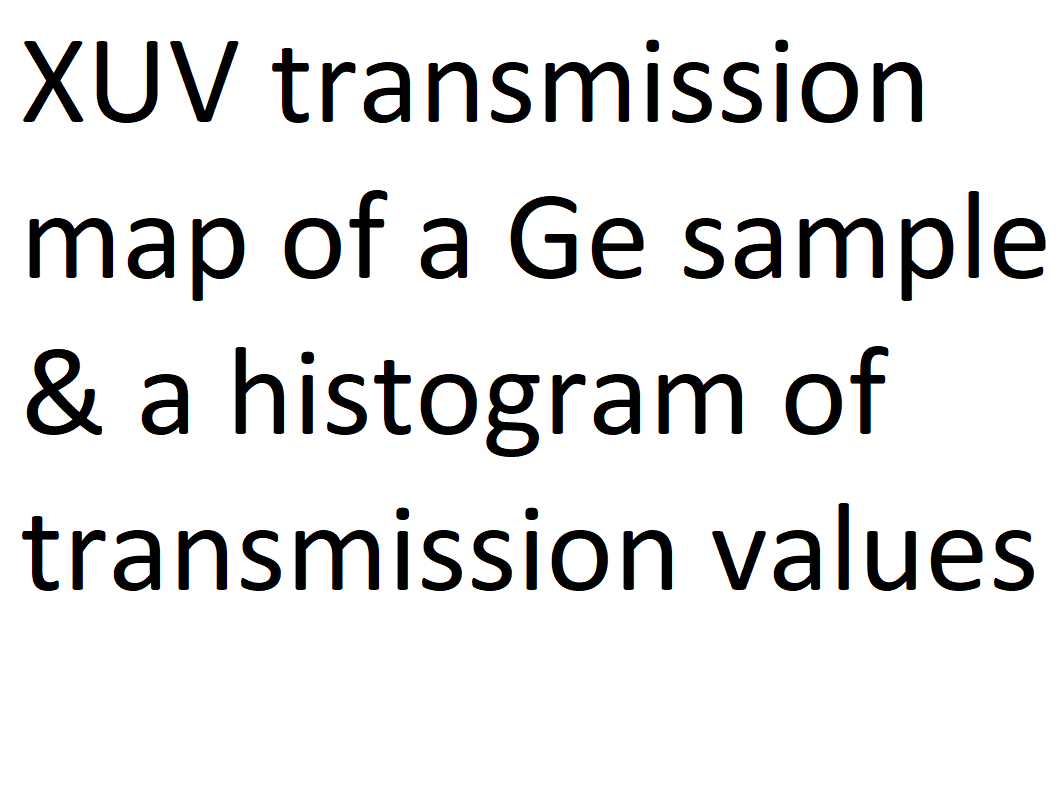
\includegraphics[width=0.5\textwidth]{figures/chap3/Ge_sample_map.png}
	\caption{this is an XUV transmission map of a germanium sample, along with a histogram of the transmission values.}
	\label{fig:Ge_sample_map}
\end{figure}

\begin{figure}
	\centering
	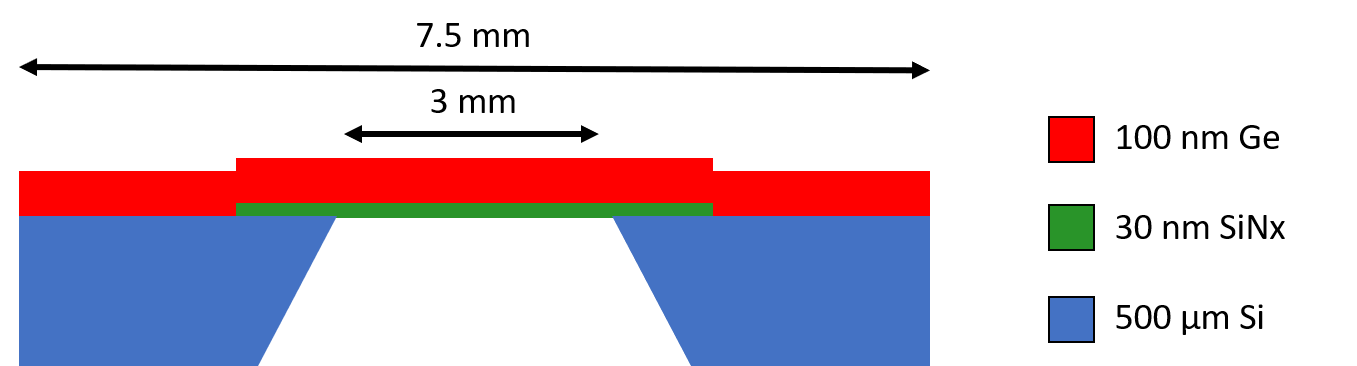
\includegraphics[width=0.75\textwidth]{figures/chap3/Sample_Geometry.png}
	\caption{Cartoon showing the cross section of the free standing sample heterostructure. A 500 $\mu$m thick Si frame supports a 30 nm low stress silicon nitride membrane (Norcada QX7300X), upon which 100 nm of germanium has been deposited. The Si frame has a 3x3 mm$^2$ clear aperture and a 7.5x7.5 mm$^2$ external dimension. The taper of the Si frame along the perimeter of the clear aperture forms a knife edge.}
	\label{fig:Sample_Geometry}
\end{figure}

\begin{figure}
	\centering
	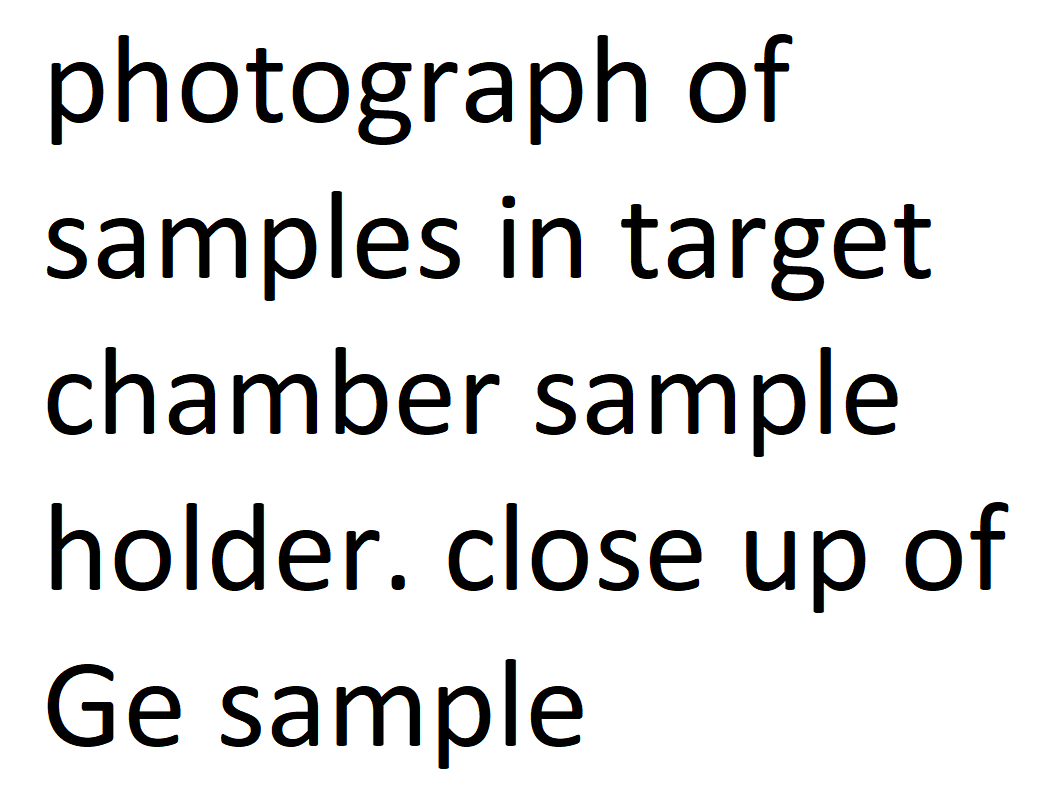
\includegraphics[width=0.5\textwidth]{figures/chap3/Samples_in_holder.png}
	\caption{photograph of the samples inside the target chamber's holder.}
	\label{fig:Samples_in_holder}
\end{figure}

The experiment consists of a series of two-dimensional images of harmonic spectra. The 


delta-OD math


experimental design: differential measurement (pump on, pump off), rastering, etc.

damage thresholds, sample thickness, sample uniformity

Ge-specific experimental parameters: wavelength, generation conditions, exposure time, MCP settings, rep rate, etc.




\section{Data Processing}

\begin{figure}
	\centering
	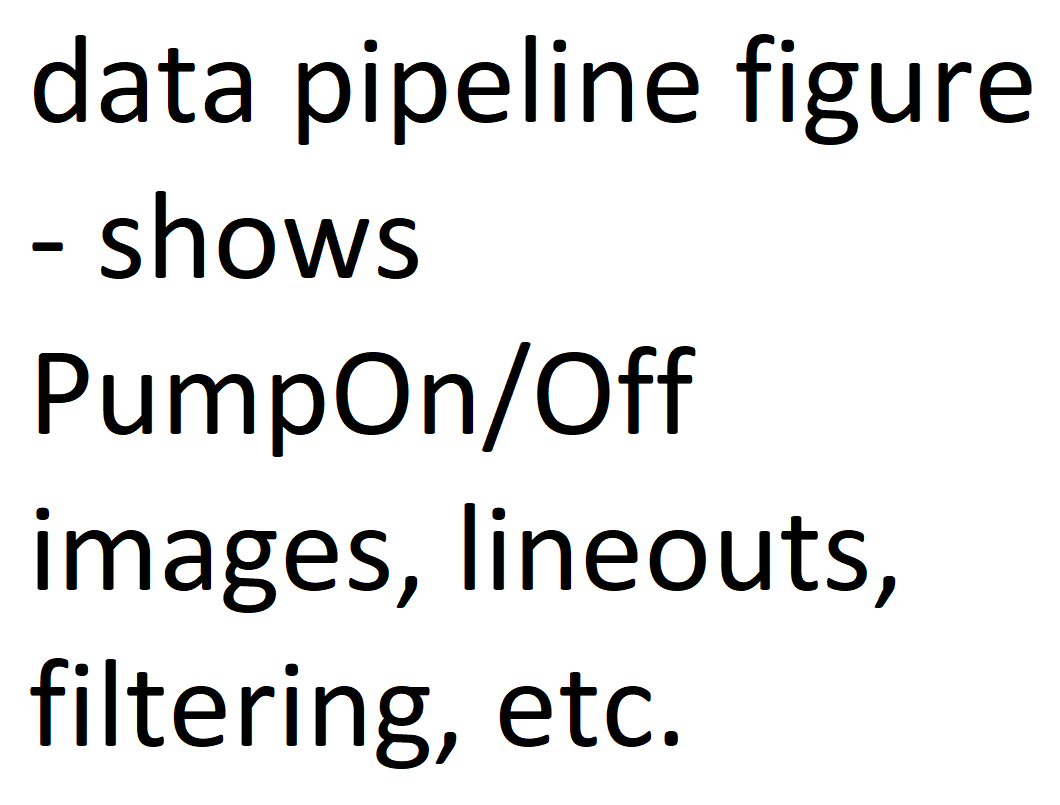
\includegraphics[width=0.5\textwidth]{figures/chap3/Data_Pipeline.png}
	\caption{this figure shows the data processing pipeline. it shows how we start with PumpOn-Off 2D images and transform them into spectrograms. it includes steps like OD calculation, spectral lineouts, frequency filtering and smooth, energy calibration, etc.}
	\label{fig:Data_Pipeline}
\end{figure}

\begin{figure}
	\centering
	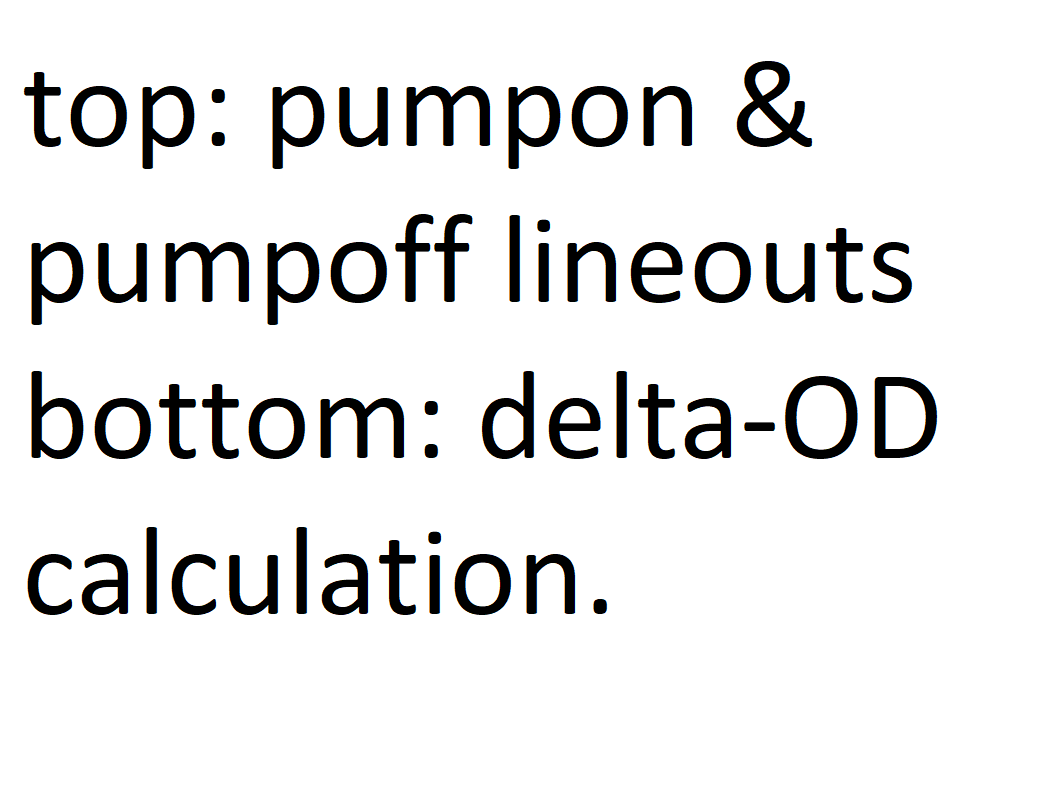
\includegraphics[width=0.5\textwidth]{figures/chap3/PumpOn_vs_PumpOff.png}
	\caption{this figure shows, using real data, a pump off and pump on spectral lineout. in another panel, it shows the delta-OD.}
	\label{fig:PumpOn_vs_PumpOff}
\end{figure}


mention calibration of spectrometer in passing, 2D image --> 1D spectrum

definition of delta-OD:

\begin{equation}
\Delta OD(E,\tau) = -\log_{10} \left(\frac{S_{sig}(E,\tau)}{S_{ref}(E)} \right)
\label{eqn:delta-OD}
\end{equation}
